\begin{figure}[h]
\centering
\subfigure[SNR = 5dB]{
	% This file was created with tikzplotlib v0.10.1.
	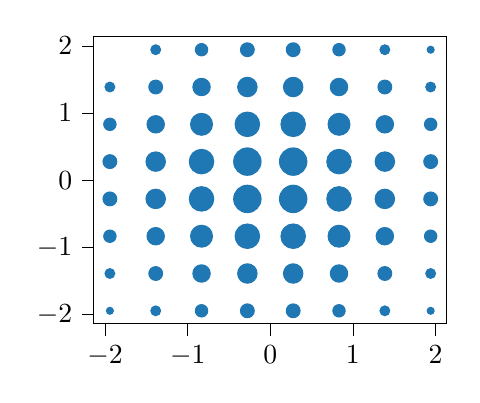
\begin{tikzpicture}
	
	\definecolor{darkgray176}{RGB}{176,176,176}
	\definecolor{steelblue31119180}{RGB}{31,119,180}
	
	\begin{axis}[
	width=0.5\columnwidth,
	tick align=outside,
	tick pos=left,
	x grid style={darkgray176},
	xmin=-2.13620593547821, xmax=2.13620593547821,
	xtick style={color=black},
	y grid style={darkgray176},
	ymin=-2.13620593547821, ymax=2.13620593547821,
	ytick style={color=black}
	]
	\addplot [
	  mark=*,
	  only marks,
	  scatter,
	  scatter/use mapped color={
	    draw=steelblue31119180,
	    fill=steelblue31119180,
	  },
	  scatter/@pre marker code/.append style={/tikz/mark size=\perpointmarksize},
	  visualization depends on={\thisrow{sizedata} \as\perpointmarksize},
	  table/row sep=\\
	]
	table{%
	x  y  sizedata
	-1.94200539588928 1.94200539588928 1.2521708\\
	-1.38714671134949 1.94200539588928 1.7632555\\
	-0.832288026809692 1.94200539588928 2.2239556\\
	-0.277429342269897 1.94200539588928 2.4847505\\
	0.277429342269897 1.94200539588928 2.4847505\\
	0.832288026809692 1.94200539588928 2.2239556\\
	1.38714671134949 1.94200539588928 1.7632555\\
	1.94200539588928 1.94200539588928 1.2521708\\
	-1.94200539588928 1.38714671134949 1.7632555\\
	-1.38714671134949 1.38714671134949 2.4829438\\
	-0.832288026809692 1.38714671134949 3.1316829\\
	-0.277429342269897 1.38714671134949 3.4989233\\
	0.277429342269897 1.38714671134949 3.4989233\\
	0.832288026809692 1.38714671134949 3.1316829\\
	1.38714671134949 1.38714671134949 2.4829438\\
	1.94200539588928 1.38714671134949 1.7632555\\
	-1.94200539588928 0.832288026809692 2.2239556\\
	-1.38714671134949 0.832288026809692 3.1316829\\
	-0.832288026809692 0.832288026809692 3.9499235\\
	-0.277429342269897 0.832288026809692 4.413116\\
	0.277429342269897 0.832288026809692 4.413116\\
	0.832288026809692 0.832288026809692 3.9499235\\
	1.38714671134949 0.832288026809692 3.1316829\\
	1.94200539588928 0.832288026809692 2.2239556\\
	-1.94200539588928 0.277429342269897 2.4847505\\
	-1.38714671134949 0.277429342269897 3.4989233\\
	-0.832288026809692 0.277429342269897 4.413116\\
	-0.277429342269897 0.277429342269897 4.9306254\\
	0.277429342269897 0.277429342269897 4.9306254\\
	0.832288026809692 0.277429342269897 4.413116\\
	1.38714671134949 0.277429342269897 3.4989233\\
	1.94200539588928 0.277429342269897 2.4847505\\
	-1.94200539588928 -0.277429342269897 2.4847505\\
	-1.38714671134949 -0.277429342269897 3.4989233\\
	-0.832288026809692 -0.277429342269897 4.413116\\
	-0.277429342269897 -0.277429342269897 4.9306254\\
	0.277429342269897 -0.277429342269897 4.9306254\\
	0.832288026809692 -0.277429342269897 4.413116\\
	1.38714671134949 -0.277429342269897 3.4989233\\
	1.94200539588928 -0.277429342269897 2.4847505\\
	-1.94200539588928 -0.832288026809692 2.2239556\\
	-1.38714671134949 -0.832288026809692 3.1316829\\
	-0.832288026809692 -0.832288026809692 3.9499235\\
	-0.277429342269897 -0.832288026809692 4.413116\\
	0.277429342269897 -0.832288026809692 4.413116\\
	0.832288026809692 -0.832288026809692 3.9499235\\
	1.38714671134949 -0.832288026809692 3.1316829\\
	1.94200539588928 -0.832288026809692 2.2239556\\
	-1.94200539588928 -1.38714671134949 1.7632555\\
	-1.38714671134949 -1.38714671134949 2.4829438\\
	-0.832288026809692 -1.38714671134949 3.1316829\\
	-0.277429342269897 -1.38714671134949 3.4989233\\
	0.277429342269897 -1.38714671134949 3.4989233\\
	0.832288026809692 -1.38714671134949 3.1316829\\
	1.38714671134949 -1.38714671134949 2.4829438\\
	1.94200539588928 -1.38714671134949 1.7632555\\
	-1.94200539588928 -1.94200539588928 1.2521708\\
	-1.38714671134949 -1.94200539588928 1.7632555\\
	-0.832288026809692 -1.94200539588928 2.2239556\\
	-0.277429342269897 -1.94200539588928 2.4847505\\
	0.277429342269897 -1.94200539588928 2.4847505\\
	0.832288026809692 -1.94200539588928 2.2239556\\
	1.38714671134949 -1.94200539588928 1.7632555\\
	1.94200539588928 -1.94200539588928 1.2521708\\
	};
	\end{axis}
	
	\end{tikzpicture}
}
\subfigure[SNR = 18dB]{
	% This file was created with tikzplotlib v0.10.1.
	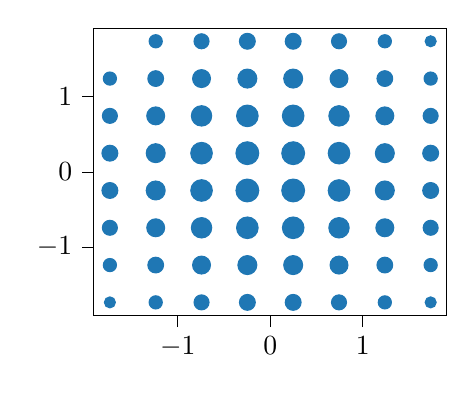
\begin{tikzpicture}
	
	\definecolor{darkgray176}{RGB}{176,176,176}
	\definecolor{steelblue31119180}{RGB}{31,119,180}
	
	\begin{axis}[
	width=0.5\columnwidth,
	tick align=outside,
	tick pos=left,
	x grid style={darkgray176},
	xmin=-1.90730187892914, xmax=1.90730187892914,
	xtick style={color=black},
	y grid style={darkgray176},
	ymin=-1.90730187892914, ymax=1.90730187892914,
	ytick style={color=black}
	]
	\addplot [
	  mark=*,
	  only marks,
	  scatter,
	  scatter/use mapped color={
	    draw=steelblue31119180,
	    fill=steelblue31119180,
	  },
	  scatter/@pre marker code/.append style={/tikz/mark size=\perpointmarksize},
	  visualization depends on={\thisrow{sizedata} \as\perpointmarksize},
	  table/row sep=\\
	]
	table{%
	x  y  sizedata
	-1.73391079902649 1.73391079902649 1.9902518\\
	-1.23850774765015 1.73391079902649 2.3760042\\
	-0.743104636669159 1.73391079902649 2.7039983\\
	-0.247701555490494 1.73391079902649 2.8618598\\
	0.247701555490494 1.73391079902649 2.8618598\\
	0.743104636669159 1.73391079902649 2.7039983\\
	1.23850774765015 1.73391079902649 2.3760042\\
	1.73391079902649 1.73391079902649 1.9902518\\
	-1.73391079902649 1.23850774765015 2.3760042\\
	-1.23850774765015 1.23850774765015 2.8365235\\
	-0.743104636669159 1.23850774765015 3.2280898\\
	-0.247701555490494 1.23850774765015 3.416548\\
	0.247701555490494 1.23850774765015 3.416548\\
	0.743104636669159 1.23850774765015 3.2280898\\
	1.23850774765015 1.23850774765015 2.8365235\\
	1.73391079902649 1.23850774765015 2.3760042\\
	-1.73391079902649 0.743104636669159 2.7039983\\
	-1.23850774765015 0.743104636669159 3.2280898\\
	-0.743104636669159 0.743104636669159 3.6737092\\
	-0.247701555490494 0.743104636669159 3.8881829\\
	0.247701555490494 0.743104636669159 3.8881829\\
	0.743104636669159 0.743104636669159 3.6737092\\
	1.23850774765015 0.743104636669159 3.2280898\\
	1.73391079902649 0.743104636669159 2.7039983\\
	-1.73391079902649 0.247701555490494 2.8618598\\
	-1.23850774765015 0.247701555490494 3.416548\\
	-0.743104636669159 0.247701555490494 3.8881829\\
	-0.247701555490494 0.247701555490494 4.115178\\
	0.247701555490494 0.247701555490494 4.115178\\
	0.743104636669159 0.247701555490494 3.8881829\\
	1.23850774765015 0.247701555490494 3.416548\\
	1.73391079902649 0.247701555490494 2.8618598\\
	-1.73391079902649 -0.247701555490494 2.8618598\\
	-1.23850774765015 -0.247701555490494 3.416548\\
	-0.743104636669159 -0.247701555490494 3.8881829\\
	-0.247701555490494 -0.247701555490494 4.115178\\
	0.247701555490494 -0.247701555490494 4.115178\\
	0.743104636669159 -0.247701555490494 3.8881829\\
	1.23850774765015 -0.247701555490494 3.416548\\
	1.73391079902649 -0.247701555490494 2.8618598\\
	-1.73391079902649 -0.743104636669159 2.7039983\\
	-1.23850774765015 -0.743104636669159 3.2280898\\
	-0.743104636669159 -0.743104636669159 3.6737092\\
	-0.247701555490494 -0.743104636669159 3.8881829\\
	0.247701555490494 -0.743104636669159 3.8881829\\
	0.743104636669159 -0.743104636669159 3.6737092\\
	1.23850774765015 -0.743104636669159 3.2280898\\
	1.73391079902649 -0.743104636669159 2.7039983\\
	-1.73391079902649 -1.23850774765015 2.3760042\\
	-1.23850774765015 -1.23850774765015 2.8365235\\
	-0.743104636669159 -1.23850774765015 3.2280898\\
	-0.247701555490494 -1.23850774765015 3.416548\\
	0.247701555490494 -1.23850774765015 3.416548\\
	0.743104636669159 -1.23850774765015 3.2280898\\
	1.23850774765015 -1.23850774765015 2.8365235\\
	1.73391079902649 -1.23850774765015 2.3760042\\
	-1.73391079902649 -1.73391079902649 1.9902518\\
	-1.23850774765015 -1.73391079902649 2.3760042\\
	-0.743104636669159 -1.73391079902649 2.7039983\\
	-0.247701555490494 -1.73391079902649 2.8618598\\
	0.247701555490494 -1.73391079902649 2.8618598\\
	0.743104636669159 -1.73391079902649 2.7039983\\
	1.23850774765015 -1.73391079902649 2.3760042\\
	1.73391079902649 -1.73391079902649 1.9902518\\
	};
	\end{axis}
	
	\end{tikzpicture}
}
\caption{Learnt probabilistic constellation shaping for M = 64. The size of the markers is proportional to the transmission probability of the symbol. When trained under 5dB, the proababilistic shaping approaches a gaussian. While under 18dB it approaches a uniform distribution. }
\end{figure}
